\documentclass[runningheads,a4paper]{llncs}
\usepackage{amssymb}
\setcounter{tocdepth}{3}
\usepackage{graphicx}
\usepackage{multirow}
\usepackage{booktabs}
\usepackage{algorithm2e}
\usepackage{url, listings, color}
%\usepackage{hyperref}

%two column float page must be 90% full
\renewcommand\dblfloatpagefraction{.99}
%two column top float can cover up to 80% of page
\renewcommand\dbltopfraction{.99}
%float page must be 90% full
\renewcommand\floatpagefraction{.99}
%top float can cover up to 80% of page
\renewcommand\topfraction{.99}
%bottom float can cover up to 80% of page
\renewcommand\bottomfraction{.99}
%at least 10% of a normal page must contain text
\renewcommand\textfraction{.01}

\newcommand{\code}[1] {{\footnotesize\sffamily #1}}

\titlerunning{SECT-AIR: Software Engineering Costs and Timescales — Aerospace Initiative for Reduction}
\authorrunning{SECT-AIR Consortium Partners}

\begin{document}

\title{SECT-AIR: Software Engineering Costs and Timescales --�� Aerospace Initiative for Reduction}

\author{Richard F. Paige$^{1}$, Athanasios Zolotas$^{1}$ Dimitrios S. Kolovos$^{1}$, \\ John A. McDermid$^{1}$,
Mike Bennett$^{2}$, Stuart Hutchesson$^{2}$, Andrew Hawthorn$^{3}$\\%
%
\footnotesize{
\{richard.paige, thanos.zolotas, dimitris.kolovos, john.mcdermid\}@york.ac.uk, \\
\{mike.bennett, stuart.hutchesson\}@rolls-royce.com\\
andrew.hawthorn@altran.com
}
%
\institute{
$^{1}$University of York, United Kingdom,\\
$^{2}$Rolls-Royce, United Kingdom,\\
$^{3}$Altran Praxis, United Kingdom
}}

\maketitle

\begin{abstract}
Software is critical to the majority of functionality in avionics and aerospace systems. The amount of safety-related software in avionics is growing rapidly (doubling in size around every four years), and the costs of software programmes in industry are increasingly unaffordable -- safety-related code can cost upwards of USD \$150 per line. At the same time, demands from avionics customers for increased scope and new functionality is increasing, and quality is non-negotiable: it is fixed by standards and safety requirements. The SECT-AIR project is addressing these cost and demand issues by focusing on automation in software engineering, with particular emphasis on model-based development. In this paper we provide an overview of the motivation behind the project, which started in 2016, and some of the key tasks it will carry out to help improve productivity, increase customer scope and maintain quality.
\end{abstract}

\section{Project Identity}

\newcommand{\bitem}[1]{\item \textbf{#1:}}

\begin{itemize}
	\bitem{Project acronym} SECT-AIR
	\bitem{Project title} Software Engineering Costs and Timescales ? Aerospace Initiative for Reduction
	\bitem{Project partners} Rolls-Royce (Coordinator), BAE Systems, Leonardo, GE Aviation, MBDA, Rapita Systems, Altran Praxis, Cobham, D-RisQ, University of York, University of Oxford, University of Southampton 
	\bitem{Website} \url{http://www.ati.org.uk/atifundedprojects/113099/} 
	\bitem{Funding} Aerospace Technology Institute/Innovate UK, total budget GBP 10.1M.
	\bitem{Project start date/duration} July 1, 2016 (36 months)
\end{itemize}

\section{Introduction}
\label{sec:introduction}

The majority of functionality in modern aerospace and avionics systems critically depends on software. Unlike other software domains, where tradeoffs between cost and quality can be made, quality requirements for avionics software systems are non-negotiable, fixed by standards such as DO-178C. As such, cost reductions for software have to be addressed by productivity improvements. One way to increase productivity is to better automate different engineering tasks, focusing on automating those tasks that are error-prone or repetitive, allowing engineers to focus on the challenging and creative aspects. Specific challenges that could be addressed to increase productivity and automation in avionics software engineering include:
\begin{itemize}
\item exploiting advanced architectures that support open and modular systems construction, e.g., service-oriented architectures, with the intent on reducing the burden of certification;
\item optimising the development process via enhanced automated testing techniques and streamlining the handover between systems and software engineering;
\item enhancing exploitation of model-based development, automated code generation, model-to-model transformation and automated formal analysis based on standards, so as to share development infrastructure costs and enable easier exchange of engineering artefacts;
\item improving development processes for building high-integrity devices, e.g., FPGAs, system-on-chip, multicore.
\end{itemize}
At the same time, these challenges need to be addressed in a way that makes them ready to adopt by the avionics industry, taking into account the requirements for certification.

This paper discusses how the SECT-AIR project has contributed to tackling these challenges. 
Section \ref{sec:execution} provides an overview of the overall SECT-AIR project execution. Section \ref{sec:work-packages} outline the different work packages with some focus on the model-based development tasks. Section \ref{sec:conclusions} outlines the ongoing evaluation process and concludes the paper.



\section{Execution}
\label{sec:execution}

SECT-AIR is a project jointly funded by the industry partners and the Aerospace Technology Institute (ATI) via Innovate UK, the UK's innovation agency. As a result, the project's operation is overseen by both a project management team (led by Rolls-Royce) and an Innovate UK Program Manager, who monitors and assesses progress against key performance indicators, technical plans and financial plans. The project's overall execution is guided by the following key principles:
\begin{itemize}
\item Developing an industry-led aerospace sector wide strategy for software engineering;
\item Exploiting technology used in other domains (e.g., high performance computing, multi- and many-core) in the aerospace domain;
\item Validating research results using robust industrial aerospace case studies from project partners;
\item Aligning industry development needs with academic research;
\item Delivering mature technologies and processes at a high technical readiness level;
\item Engaging with certification authorities, so as to be sure that the technologies and solutions produced will lead to systems that can realistically achieve certification. To support this, SECT-AIR will engage with the Civil Aviation Authority.
\end{itemize}
The overriding focus in all of the research projects (carried out in the work packages, described in the next section) is on automation as a means to improve productivity. Success measures in the case studies will be based on increases in automation in different processes.






\section{Work Packages}
\label{sec:work-packages}

Figure~\ref{fig:wps} shows the work package breakdown for SECT-AIR, including their interrelationships. 

\begin{figure}[htbp]
\centerline{\scalebox{0.7}{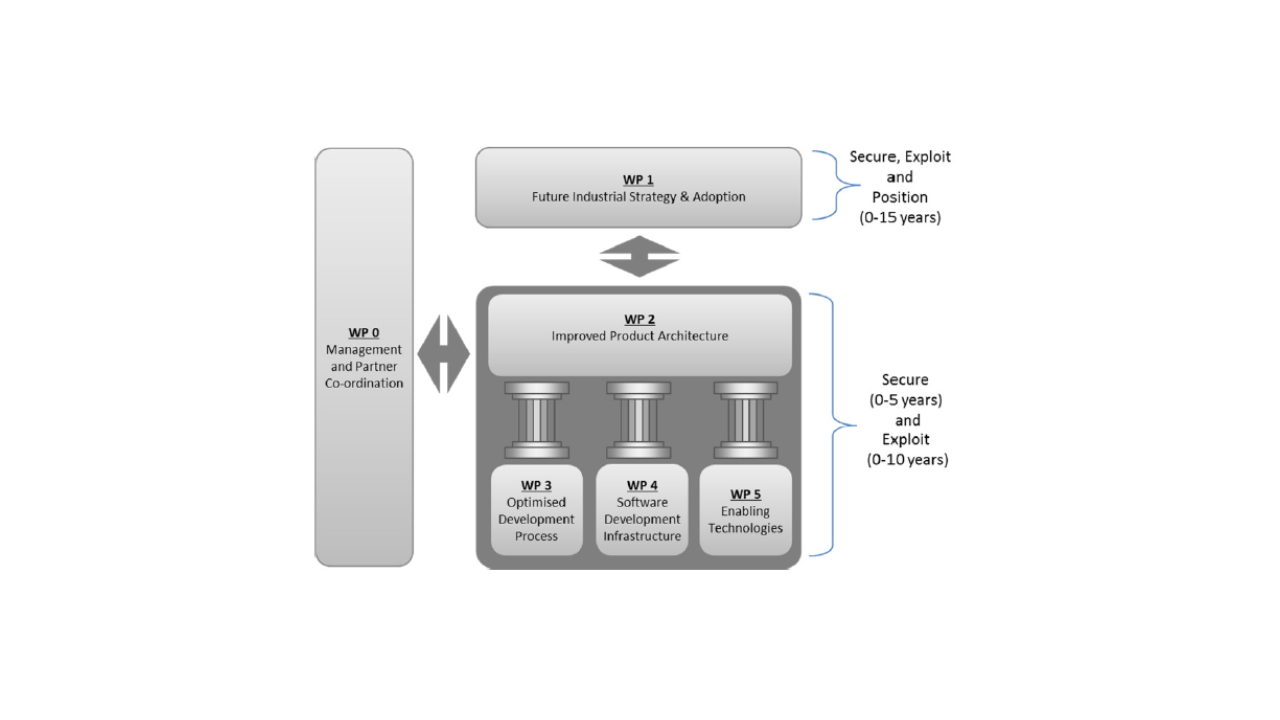
\includegraphics{work-packages.png}}}
\caption{Work package structure for SECT-AIR}
\label{fig:wps}
\end{figure}

Work Package (WP1) focuses
on industry strategy and adoption of SECT-AIR deliverables: it includes baselining activities to measure current state of practice in aerospace software engineering, and will
support experiments designed to demonstrate potential improvements. It also aims to create a long-term industry strategy (for 10-15 years)
that will ensure significant industry and academic alignment. It will be responsible for coordinating usable case study material for research in other work
packages.

WP2 focuses on developing a common open and modular product architecture for aerospace software engineering, which will in turn enhance the product
supply chain. It will also investigate the use of partitioning in aerospace products to reduce the amount of safety-critical functionality within embedded products.
It will deliver demonstrators of open architectures at high technical readiness levels. The open architecture will be evaluated via demonstrator case studies that
will be identified in WP1.

WP3 investigates software development processes. It is particularly targeting the application and evaluation of model-based techniques for requirements
specification, to ensure composability and reuse of requirements: the view is that across a number of aerospace projects (requiring certification) there is a significant opportunity to reuse requirements -- especially if they can be captured in a standard and tool-supported modelling language. As well, WP3 will investigate traceability and will build a toolchain to support end-to-end
traceability from requriements models through to documentation and code. WP3 will in parallel trial the application of formal specification techniques used in
synergy with model-based techniques to support richer analysis of requirements. The techniques that are developed will be applied to case studies that
focus on novel interactive interfaces, e.g., for cockpit display systems. Such systems benefit from the development of rapid prototypes (even for critical
systems) and thus make a challenging case study for model-based and formal methods, especially given that minimising the cost and time to change,
for example, display formats, is an industry-wide issue in aerospace.

WP4 focuses on software development infrastructure for aerospace software engineering. It will endeavour to set a UK strategy for software development
infrastructure improvements, and  develop tool support to provide integration to various model-based languages used by industry, e.g., SysML, UML and
various UML profiles such as MARTE. It will also aim to reduce the overhead for code-level verification and for generating qualification and assurance data.
We discuss WP4 in more detail in the next subsection.

WP5, Enabling Technologies, aims to deliver a roadmap and demonstrator for next-generation high-performance obsolescence protected platforms. In particular
it will aim to reduce the effort and costs for producing high-integrity firmware, such as system-on-chip and many-core processors. It will also work with certification
authorities to ensure that the best practice that is developed will lead to systems that can achieve certification. A particular technique that will be investigated will
be modular component-based development.

\subsection{Model-based development}
WP4 broadly focuses on software development infrastructure -- i.e., producing a common platform (largely via reuse and agreement on standards) -- for aerospace
software engineering. The vision is to exploit model-based development techniques as a means to increase productivity and to automate the error-prone, repetitive
and tedious tasks of engineers. There are three components to achieving this vision:
\begin{itemize}
\item Exploiting model-based languages, including general-purpose languages (and tools) as well as techniques for building domain-specific languages for specific problems. 
There is broad agreement on the use of (profiles of) UML and SysML throughout SECT-AIR, and the project partners have predominantly agreed on the use of Eclipse
Papyrus for many of their modelling needs within the project. A key requirement is to support efficient and effective development of UML profiles for individual partners,
including those partners who have limited-to-no experience of building profiles. Thus, one objective of WP4 is to investigate new and efficient ways of \textit{generating}
profiles for UML and SysML, maximising reuse (e.g., when two or more profiles share features).

\item Providing support for efficient and effective model transformations. Many partners in SECT-AIR need transformations to allow them to use new modelling
technology such as Eclipse Papyrus in combination with legacy modelling technology, such as Artisan PTC Modeller. A particular objective of this work package is to
ensure that any enabling model transformation technology is efficient, even when applied to large and complicated models. As such, WP4 is investigating 
\textit{incremental} model transformations, where small changes to the source models mean that only small parts of the transformations need to be executed
again.


\item Generating text. A particular use case for generation of text is producing
template \textit{assurance cases} from engineering artefacts (e.g., UML design models). Template assurance cases provide the structure and outline of an assurance
argument that -- after refinement and instantiation -- will be delivered to a certifying authority along with evidence (e.g., test data, traceability data). Such arguments are
and evidence are critical in attempting to convince the certifying authority that a system is acceptably safe to deploy in its environment. Producing assurance cases is
generally carried out manually and is an expensive process. Recertifying a system where requirements have changed is also a very expensive process. Hence, there is strong
potential in using model-to-text transformatio to at least partly automate the process of producing assurance cases.
\end{itemize}

Case studies from industry partners focusing on security and safety-critical systems development are being identified to help demonstrate the effectiveness
of the techniques developed in this work package.






\section{Evaluation and Conclusions}
\label{sec:conclusions}

In this paper, we have given an overview of the SECT-AIR project, which aims to reduce software cost to the UK aerospace industry. The state of play is that the cost of software for aerospace is damaging the industry, and both industry and academia must collaborate in order to introduce controls, increase productivity and hence lower costs. SECT-AIR has been designed to bring together key UK capability in development of high-integrity aerospace software.

SECT-AIR has been running since June 2016 and already has delivered a number of results, including baselining surveys and experiments to establish cross-industry state of practice, an analysis of the use of model transformation across the industry, and the development of driver technology to allow SECT-AIR partners to use modern model management technology (i.e., Epsilon and its transformation language \cite{Kolovos2008}) with legacy modelling tools (e.g., PTC Integrity Modeller). The focus over the next six months will be on leveraging these results to support the industry partners in more efficient development of their own profiles of UML and SysML, and on automating the generation of evidence that would be used as part of an assurance case for a high-integrity system.

% \subsection*{Acknowledgements}
% We would like to thank Scott Hansen (The Open Group), Alessandra Bagnato (SOFTEAM), Pedro Mal\'o (Uninova), Vincent Hanniet (Soft-Maint) and Salvator Trujillo (IKERLAN) for their help with identifying the challenges related to scalable MDE from an industrial perspective, and for their contributions to shaping the proposed research directions.

\paragraph*{}\textbf{Acknowledgements} This work was supported by the Aerospace Technology Institute and Innovate UK via the SECT-AIR grant, project number 113099.

\bibliographystyle{unsrt}
\bibliography{bibliography}  % sigproc.bib is the name of the Bibliography 

\end{document}
